%% open-cam IQ lab: IS&T Electronic Imaging 2027 companion paper (draft).
%% Build: see README.md. Numbers come from tables/*.tex, written by scripts/make_tables.py.
\documentclass[letterpaper,twocolumn,fleqn]{article}
\usepackage{ist}
\usepackage{microtype}
\usepackage{booktabs}
\usepackage{graphicx}
\usepackage{amsmath}
\usepackage{url}
\usepackage[hidelinks]{hyperref}
\emergencystretch=1.5em

%% Generated by scripts/make_tables.py -- do not edit.
\newcommand{\deBest}{1.25}
\newcommand{\deBestRecipe}{\texttt{default\_quad\_bayer}}
\newcommand{\deMedian}{2.83}
\newcommand{\deUnderTwo}{22}
\newcommand{\deWorst}{12.95}
\newcommand{\deWorstRecipe}{\texttt{default\_rgb\_noircf}}
\newcommand{\drMedDcg}{80.8}
\newcommand{\drMedLinear}{74.3}
\newcommand{\drMedLofic}{93.1}
\newcommand{\drMedMultiexposure}{118.8}
\newcommand{\drMedSplitpixel}{104.4}
\newcommand{\drOneMax}{118.8}
\newcommand{\drOneMin}{62.3}
\newcommand{\glareMax}{0.08}
\newcommand{\glareMin}{0.00}
\newcommand{\mtfMax}{0.500}
\newcommand{\mtfMin}{0.112}
\newcommand{\mtfSensorMax}{0.414}
\newcommand{\mtfSensorMin}{0.158}
\newcommand{\nFailed}{0}
\newcommand{\nGroups}{13}
\newcommand{\nRebound}{4}
\newcommand{\nRecipes}{84}
\newcommand{\nScored}{84}
\newcommand{\reboundLimit}{0.5}
\newcommand{\scRes}{480$\times$320}
\newcommand{\scSpp}{64}
\newcommand{\texMax}{3.45}
\newcommand{\texMin}{0.44}
\newcommand{\valCases}{75}
\newcommand{\valFailures}{0}
\newcommand{\valSharpBias}{3.2}


\title{An image-quality laboratory for spectral camera simulation: ground-truth-validated metrics and a scorecard of \nRecipes{} camera recipes}

\author{Brian Deegan;
        University of Galway;
        Galway, Ireland}

\date{}

\begin{document}
\maketitle
\thispagestyle{empty}

\begin{abstract}
Camera simulators are increasingly used to compare sensors, lenses and pixel architectures before hardware exists, but such comparisons are only as trustworthy as the image-quality (IQ) metrics applied to the simulated images. We present the IQ lab of open-cam, an open-source spectral camera simulator built on pbrt-v4. It provides four procedurally generated test scenes (an emissive 120\,dB HDR chart, a tabletop diorama, a skin-tone chart and an ISO~18844-style black-hole flare target) and metrics for SNR, dynamic range, IEEE~P2020 contrast detection probability (CDP), slanted-edge and dead-leaves acutance, CIEDE2000 colour error and veiling glare. Before using the metrics on renders, we validate each against synthetic inputs with closed-form answers: all \valCases{} cases pass explicit tolerances, and the one systematic bias found (sharp edges read MTF50 up to \valSharpBias\,\% low) is traced to the ISO~12233 default 4$\times$ edge binning. We then score every one of the \nRecipes{} camera recipes shipped with open-cam on all four scenes through the full spectral pipeline, sharing pbrt renders across the \nGroups{} distinct optical configurations. We describe the measurement decisions that the scorecard forced, which apply equally to any simulated IQ study: locating ROIs through real lens distortion, metering on the chart rather than the scene, and separating sensor noise from Monte-Carlo render noise.
\end{abstract}

\section{Introduction}
Simulation lets an imaging engineer ask how a dual-conversion-gain pixel, a different colour filter array (CFA) or a faster lens changes image quality long before a sample exists. Image-systems simulators such as ISETCam~\cite{farrell2012digital,isetcam} and open-cam~\cite{opencam} carry light in physical, spectral units through the optics into photoelectrons, so the simulated raw data obey the same photon statistics as a real sensor. What is less often discussed is the last step: the IQ metrics applied to the simulated images. Standardised metrics, for example ISO~12233 resolution~\cite{iso12233}, ISO~15739 noise~\cite{iso15739}, ISO~19567-2 texture~\cite{iso19567}, ISO~18844 flare~\cite{iso18844}, CPIQ acutance~\cite{baxter2012cpiq} and the IEEE~P2020 automotive KPIs~\cite{p2020whitepaper,geese2018cdp}, were written for physical test charts in a laboratory. Applying them to renders raises questions that a laboratory does not: is a metric biased on a perfectly noise-free input; does Monte-Carlo render noise masquerade as sensor noise; and where, in pixels, is a chart patch once a real lens prescription has distorted the image?

This paper describes the open-cam IQ lab and its use to compare all camera recipes in the repository. Its contributions are (i) a set of procedurally generated, asset-free pbrt-v4 test scenes and NumPy metrics for SNR, dynamic range, CDP, acutance, colour and flare; (ii) a ground-truth validation suite that tests every metric against closed-form answers with explicit tolerances; (iii) a recipe scorecard that runs every scene through the full spectral sensor pipeline of every recipe; and (iv) an account of the measurement pitfalls the scorecard exposed and how they were resolved. Everything, including the scripts that produce every number in this paper, is in the open-cam repository.

\section{Test scenes and metrics}
All scenes are generated by Python builders that write pbrt-v4 scene files plus a JSON description of every region of interest (ROI). They need no external assets, so a scene can be regenerated at any resolution.

\textbf{HDR chart.} Twenty-one log-spaced diffuse area emitters span 120\,dB in 6\,dB steps on a zero-reflectance background. Each patch is split: the left half (luminance $L$) gives signal and noise, and the right half ($L(1+C)/(1-C)$, $C=0.2$) gives every level a fixed Michelson contrast for CDP. Because there is no inter-patch light transport, each ROI sees its patch's radiance exactly.

\textbf{Diorama.} A tabletop scene combines a spectral 24-patch ColorChecker, a skin-tone chart, a dead-leaves card, a Siemens star and a 5$^\circ$ slanted edge with matte, glossy, metal and glass spheres, a 6500\,K window roughly 700$\times$ brighter than the shadowed wall and a 2700\,K bulb. It exercises colour, sharpness, texture and scene dynamic range in one frame.

\textbf{Skin chart.} Twelve patches: eight synthetic tones, the measured ColorChecker light and dark skin, a 90\,\% white and an 18\,\% grey. The synthetic tones apply a melanosome absorption power law, $R = R_{\mathrm{base}}\exp(-\tau(\lambda/500\,\mathrm{nm})^{-3.33})$~\cite{jacques2013optical}, to the measured light-skin reflectance, giving individual typology angles~\cite{chardon1991ita} from about $+61^\circ$ to $-33^\circ$ under D65. They are physically motivated but are not measured population data.

\textbf{Flare target.} An ISO~18844-style uniform emissive field with nine zero-reflectance holes at the centre, 0.7 and 0.75 field. Veiling glare is $100\times$(hole core mean $-$ true hole radiance)/(mean of the surrounding ring); the holes are found in the image itself, so the metric works through distortion and on real captures.

\textbf{Metrics.} SNR is computed on plane-detrended patches, or temporally from two frames; dynamic range (DR) is the ratio of the saturation level to the signal at which SNR falls to 1 (EMVA1288 style~\cite{emva1288std}) or 10 (ISO~15739 style). CDP is the probability that the Michelson contrast of a random dark/bright pixel pair lies within $\pm50\,\%$ of the nominal contrast~\cite{geese2018cdp}. Slanted-edge MTF follows ISO~12233~\cite{iso12233,williams2003lowfreq}; texture MTF is $\sqrt{(\mathrm{PSD}_{\mathrm{capture}}-\mathrm{PSD}_{\mathrm{noise}})/\mathrm{PSD}_{\mathrm{ideal}}}$, radially averaged~\cite{cao2009texture}, which in simulation needs no analytic dead-leaves model because the ideal target is known exactly. Acutance weights the MTF by the CPIQ contrast sensitivity function for a given viewing geometry~\cite{baxter2012cpiq}. Colour error is CIEDE2000~\cite{sharma2005ciede2000}, with the chart's own white patch as reference white. IEEE~P2020 and CPIQ are not open documents, so these are implementations from the published papers and ISO structure, not certified ones; all constants are exposed as arguments.

\section{Ground-truth validation}
Each metric is first tested on synthetic inputs whose answer is known in closed form, over several noise realisations, and the bias and spread are checked against explicit tolerances (Table~\ref{tab:val}). Edges at 3, 5 and 8$^\circ$ are blurred by a Gaussian of $\sigma=0.5$--2\,px on an 8$\times$ grid and box-averaged into pixels, so the true MTF is $\exp(-2\pi^2\sigma^2f^2)|\mathrm{sinc}\,f|$. Dead-leaves targets are blurred by known Gaussians. Poisson flats with read noise and photo-response non-uniformity have SNR $S/\sqrt{S+r^2+(pS)^2}$; clipped patch ladders give the exact SNR\,=\,1 and 10 thresholds from $S^2 = T^2(S+r^2)$; CDP is compared with a quadrature of the pair-contrast distribution; and colour patches are shifted by known $\Delta L^*$, $\Delta C^*$ and $\Delta h$. Tolerances are split into a clean tier (noise-free, or edge SNR\,$\geq$\,100), which tests bias, and a noisy tier, which tests repeatability.

\begin{table}[t]
\caption{Ground-truth validation: worst case over all configurations against the tolerance (\valCases{} cases, \valFailures{} failures; seed 0, also passing with seeds 1--3).}
\label{tab:val}
\vspace{14pt}
\centering\small
\begin{tabular}{@{}lrr@{}}
\toprule
Quantity (worst case) & Error & Limit \\
\midrule
Edge MTF50 bias, clean (\%) & 3.17 & 3.5 \\
Edge MTF50 RMS, SNR 30 (\%) & 6.51 & 8 \\
Edge acutance, clean & 0.0109 & 0.015 \\
Texture MTF RMS, clean & 0.0022 & 0.005 \\
Texture MTF RMS, noisy & 0.0396 & 0.06 \\
SNR bias, 5--5000\,e$^-$ (\%) & 0.45 & 1 \\
DR at SNR\,=\,1 / 10 (dB) & 0.22 & 0.4 \\
CDP (absolute) & 0.0029 & 0.006 \\
$\Delta E_{00}$, 2\,\% noise & 0.185 & 0.3 \\
$\Delta E_{00}$, noise-free & 8e-13 & $10^{-6}$ \\
\bottomrule
\end{tabular}

\end{table}

All cases pass. The one systematic effect is that noise-free sharp edges ($\sigma=0.5$\,px, MTF50\,$\approx$\,0.32\,cy/px) read MTF50 up to \valSharpBias\,\% low. Changing the window or the derivative correction does not remove it; raising the ESF oversampling from the ISO default of 4$\times$ to 8$\times$ reduces it to 0.4\,\%. A regression test pins this behaviour, and for very sharp optics we either oversample 8$\times$ or treat MTF50 as about 3\,\% conservative.

\section{Recipe scorecard}
open-cam ships \nRecipes{} camera recipes (phone, compact, interchangeable-lens, automotive and research cameras, plus reference HDR and CFA variants). The scorecard runs every recipe on all four scenes through the same pipeline as a normal open-cam run: a pbrt-v4 spectral render, conversion to photoelectrons with the recipe's QE and IR-cut filter, the EMVA1288-style noise model, CFA sampling, the recipe's HDR pixel architecture and ADC, demosaicing, white balance on the white patch and the recipe's spectral ColorChecker colour-correction matrix. The skin chart is never used to fit the colour correction.

\textbf{Render reuse.} The spectral render depends only on the scene and the optics, so recipes are grouped by optical configuration (lens prescription and aperture, or pinhole and thin-lens field of view). The \nRecipes{} recipes fall into \nGroups{} groups, and each scene is rendered once per group; sensor processing still runs once per recipe. Each camera is focused on the target plane and its distance scaled so that the chart fills the same fraction of the frame. The HDR chart is pinhole-only, so its DR, SNR and CDP are sensor metrics that exclude lens transmission and flare.

\textbf{ROIs through real lenses.} The builders compute ROIs by pinhole projection. For realistic lens prescriptions this placed ROIs well off their patches: patch means differed by 30--60\,\%. Instead, a 4-sample-per-pixel render with pbrt's \texttt{gbuffer} film in world coordinates~\cite{pbrtv4format} records the world-space hit point of every pixel, and each ROI is the bounding box of pixels that see the inner 70\,\% of the target's world rectangle. This accounts for distortion and pupil effects of the traced lens~\cite{kolb1995realistic} at negligible cost.

\textbf{Exposure.} The diorama contains a window and a lamp. Exposing to the 99th percentile of the scene left the cards at about 20\,e$^-$, so edge and texture metrics measured noise. The scorecard therefore spot-meters, as a laboratory would set exposure on the chart, iterating until the metered signal is within 2\,\% of its target. The target is 0.5 of the saturation level for the diorama and 0.6 for the skin chart, where saturation is the full well or the ADC ceiling if lower. Three details of the metering decided whether the sharpness and colour numbers could be trusted. (i) The diorama's practical lamp and window lit the slanted-edge card about $5\times$ brighter than the ColorChecker, and unevenly: the white side rose by about 18\,\% across the edge ROI. Metered on the ColorChecker white, the edge clipped, which hid the gradient and returned an MTF50 of about 0.43\,cy/px. Unclipped, the gradient flattened the measured MTF near 0.5, so MTF50 for the same render ranged from 0.07 to 0.20\,cy/px with the sensor-noise seed alone. The scorecard therefore lights the diorama with its uniform fill panel only, as a laboratory lights a chart (MTF50 0.34--0.40\,cy/px over four seeds), and the meter also uses the 90th percentile of the edge ROI. (ii) The meter reads the brightest demosaiced channel. Metering on the densest CFA channel let the panchromatic W of RGBW clip (skin $\Delta E_{00}$ 46 instead of 4.9). (iii) A $2\times2$ charge-binned quad-Bayer pixel keeps the photodiode's conversion gain, so its 10-bit ADC clips at about 4800\,e$^-$, not at the 19\,200\,e$^-$ binned full well (skin $\Delta E_{00}$ 43 instead of 1.4). HDR pixels are metered below their first readout transition (e.g. the DCG high-gain ceiling), so the diorama and skin chart are scored on the primary readout and the edge does not straddle a merge switch. The brightest HDR patch is placed at 90\,\% of the recipe's HDR saturation, and the flare scene uses percentile exposure.

\textbf{Sensor noise versus render noise.} A path-traced render has Monte-Carlo noise, which is fixed for a given render and is therefore indistinguishable from scene texture or from photo-response non-uniformity in a single frame. The HDR chart is captured twice with different sensor-noise seeds, and SNR and DR use the temporal noise of the two frames. Without this, Monte-Carlo noise capped the SNR of an 8-sample HDR render at about 18\,dB, and the chart is always rendered with at least 128 samples per pixel. The diorama is rendered twice with different sampler seeds (set in the scene; pbrt's \texttt{--seed} option left the image unchanged) and captured once from each. The PSD of $(I_1-I_2)/\sqrt{2}$ then contains both sensor and render noise and is subtracted from the dead-leaves PSD. With a common render the subtraction left the Monte-Carlo noise in, and texture acutance read 1.1--6.7; with independent renders it reads 0.5--0.9. Isolated Monte-Carlo fireflies on the edge card (above $1.5\times$ the white plateau) are replaced by their $3\times3$ median before the edge SFR.

\textbf{Sharpness before and after the CCM.} Edge and texture metrics are measured on the output luminance, after the recipe CCM. Several non-Bayer CFAs need large CCMs (coefficients up to about 4 for RCCB and RCCG, 14 for RGBW), and their output luminance then subtracts sparsely sampled, more blurred channels from the dense one: for RCCB, $Y\approx2.7\,C-1.35\,B-0.27\,R$. The output MTF then dips and overshoots instead of falling monotonically, so its MTF50 is not comparable with other recipes': on one capture RCCB reads 0.11\,cy/px after the CCM and 0.38\,cy/px on its clear channel. This is what an ISP that applies the CCM to every channel produces, so the scorecard keeps the output numbers, and adds two more. The MTF rebound is the largest rise of the output MTF above its running minimum below 0.5\,cy/px, and output MTF50 is flagged as not comparable when it exceeds \reboundLimit{}. Sensor MTF50 and edge acutance are measured on the brightest demosaiced channel before the CCM (G, C or W) and are comparable across CFAs.

\textbf{Binned readouts.} Recipes with charge-binned quad-Bayer readout produce a half-resolution Bayer raster. Their ROIs are scaled to the binned raster and the CFA collapses to its binned tile; scoring them on the native $4\times4$ tile left HDR patches empty.

\section{Results}
The scorecard was run at \scRes{} with \scSpp{} samples per pixel (HDR chart 960$\times$640, 128 samples); \nScored{} of \nRecipes{} recipes were scored on every scene and \nFailed{} failed. Tables~\ref{tab:hdr}--\ref{tab:skin} and Fig.~\ref{fig:sc} summarise the results; the full per-recipe table is written to \texttt{scorecard.md} alongside the JSON and CSV.

\begin{table}[t]
\caption{HDR chart by pixel architecture: number of recipes, range of DR at SNR\,=\,1 and medians of DR at SNR\,=\,10, SNR at 18\,\% of saturation and the lowest level (dB re.\ saturation) with CDP\,$\geq$\,0.9.}
\label{tab:hdr}
\vspace{14pt}
\centering\small
\begin{tabular}{@{}lrrrrr@{}}
\toprule
Architecture & $n$ & DR$_1$ range & DR$_{10}$ & SNR$_{18}$ & CDP$_{0.9}$ \\
\midrule
Linear & 80 & 62.3--86.8 & 43.6 & 34.9 & -36 \\
Dual conversion gain & 1 & 80.8 & 46.2 & 36.0 & -36 \\
LOFIC & 1 & 93.1 & 59.7 & 41.8 & -54 \\
Split pixel & 1 & 104.4 & 70.6 & 32.4 & -66 \\
Multi-exposure & 1 & 118.8 & 86.9 & 32.0 & -78 \\
\bottomrule
\end{tabular}

\end{table}

\textbf{Dynamic range.} DR at SNR\,=\,1 spans \drOneMin--\drOneMax\,dB across all recipes (Table~\ref{tab:hdr}). The linear recipes have a median of \drMedLinear\,dB, and the HDR architectures order as their design intends: dual conversion gain \drMedDcg, LOFIC \drMedLofic, split pixel \drMedSplitpixel{} and multi-exposure \drMedMultiexposure\,dB. The lowest level with CDP\,$\geq$\,0.9 extends with DR, from $-36$\,dB for the linear median to $-78$\,dB for multi-exposure. The split-pixel and multi-exposure pixels pay for their range with a lower SNR at 18\,\% of saturation (about 32\,dB against 35\,dB for the linear median), because the merge switches to a shorter or less sensitive readout below that level.

\begin{table*}[t]
\caption{Diorama and flare metrics by optical configuration (medians over the recipes sharing it). MTF50 in cycles/pixel; acutance for a 100\,\% monitor view.}
\label{tab:optics}
\vspace{14pt}
\centering\small
\begin{tabular}{@{}lrrrrr@{}}
\toprule
Optics & $n$ & MTF50 & Edge acut. & Tex. acut. & Glare \% \\
\midrule
\texttt{dgauss.50mm}, 12.34mm aperture & 26 & 0.298 & 0.80 & 0.46 & 0.01 \\
\texttt{dgauss.50mm}, 25mm aperture & 16 & 0.301 & 0.84 & 0.89 & 0.01 \\
\texttt{wide\_22mm}, 8.708mm aperture & 10 & 0.311 & 0.83 & 0.80 & 0.02 \\
\texttt{wide\_22mm}, 4mm aperture & 10 & 0.246 & 0.83 & 0.98 & 0.03 \\
\texttt{wide\_22mm}, 8.756mm aperture & 8 & 0.325 & 0.85 & 0.84 & 0.00 \\
pinhole, 45deg & 5 & 0.367 & 0.84 & 0.60 & 0.02 \\
\texttt{wide\_22mm}, 8mm aperture & 3 & 0.311 & 0.81 & 0.80 & 0.05 \\
pinhole, 35deg & 1 & 0.348 & 0.84 & 0.59 & 0.02 \\
thinlens, 35deg & 1 & 0.375 & 0.82 & 0.58 & 0.03 \\
thinlens, 47deg & 1 & 0.419 & 0.86 & 0.57 & 0.03 \\
thinlens, 20deg & 1 & 0.361 & 0.84 & 0.62 & 0.03 \\
thinlens, 75deg & 1 & 0.340 & 0.81 & 0.57 & 0.02 \\
\texttt{wide\_22mm}, 2.75mm aperture & 1 & 0.320 & 0.82 & 0.88 & 0.00 \\
\bottomrule
\end{tabular}

\end{table*}

\textbf{Sharpness and flare.} Behind the realistic lenses the median output MTF50 is 0.25--0.33\,cy/px, below the 0.34--0.42\,cy/px of the pinhole and thin-lens groups, whose only blur is the pixel aperture and demosaicing. Edge acutance varies much less (0.80--0.86 across groups), consistent with the MTF50 ripple discussed below. Over all recipes MTF50 ranges from \mtfMin{} to \mtfMax{}\,cy/px and veiling glare from \glareMin{} to \glareMax\,\% (Table~\ref{tab:optics}).

\begin{table*}[t]
\caption{Edge sharpness by CFA (medians): MTF50 of the output luminance (after the CCM), its MTF rebound, and MTF50 and edge acutance of the brightest channel before the CCM.}
\label{tab:cfa}
\vspace{14pt}
\centering\small
\begin{tabular}{@{}lrrrrr@{}}
\toprule
CFA & $n$ & MTF50 (out) & Rebound & MTF50 (sensor) & Edge acut. (sensor) \\
\midrule
\texttt{GBRG} & 74 & 0.302 & 0.19 & 0.300 & 0.83 \\
\texttt{CMY} & 1 & 0.192 & 0.49 & 0.191 & 0.70 \\
\texttt{QUAD\_BAYER} & 1 & 0.157 & 0.03 & 0.158 & 0.49 \\
\texttt{RCCB} & 1 & 0.120 & 1.06 & 0.377 & 0.86 \\
\texttt{RCCC} & 1 & 0.405 & 0.11 & 0.396 & 0.87 \\
\texttt{RCCG} & 1 & 0.500 & 0.81 & 0.370 & 0.85 \\
\texttt{RGBW} & 1 & 0.134 & 0.93 & 0.195 & 0.69 \\
\texttt{RGBW\_4X4} & 1 & 0.112 & 2.33 & 0.319 & 0.81 \\
\texttt{RGGB} & 1 & 0.346 & 0.20 & 0.338 & 0.77 \\
\texttt{RGGCY} & 1 & 0.385 & 0.26 & 0.295 & 0.75 \\
\texttt{RYYCY} & 1 & 0.299 & 0.40 & 0.373 & 0.87 \\
\bottomrule
\end{tabular}

\end{table*}

\textbf{Sharpness by CFA.} \nRebound{} recipes have an output MTF rebound above \reboundLimit{} (Table~\ref{tab:cfa}): RCCB, RCCG and both RGBW layouts. Their output MTF50 (0.11--0.50\,cy/px) reflects the CCM, not the sensor. Before the CCM, the clear channel of RCCB and RCCG reaches 0.37--0.38\,cy/px, close to the Bayer reference on the same pinhole render (0.41). Across all recipes sensor MTF50 ranges from \mtfSensorMin{} to \mtfSensorMax{}\,cy/px. The lowest values are physical: the binned quad-Bayer raster has half the sampling rate (0.16\,cy/px in full-resolution pixels), and the $2\times2$ RGBW and CMY tiles sample their brightest channel on fewer sites (0.19--0.20).

\begin{table*}[t]
\caption{Skin-tone $\Delta E_{00}$ (D65, 12 patches): the four best and four worst recipes.}
\label{tab:skin}
\vspace{14pt}
\centering\small
\begin{tabular}{@{}lrrl@{}}
\toprule
Recipe & Mean & Max & CFA \\
\midrule
\texttt{default\_quad\_bayer} & 1.25 & 2.01 & \texttt{QUAD\_BAYER} \\
\texttt{research\_realistic\_wide22\_traced\_ghosts} & 1.36 & 2.09 & \texttt{GBRG} \\
\texttt{research\_thinlens\_macro} & 1.38 & 1.74 & \texttt{GBRG} \\
\texttt{research\_realistic\_wide22} & 1.38 & 2.08 & \texttt{GBRG} \\
\texttt{leica\_m\_type\_262} & 5.36 & 6.91 & \texttt{GBRG} \\
\texttt{default\_rccg} & 5.36 & 9.29 & \texttt{RCCG} \\
\texttt{default\_rccc\_noircf} & 9.73 & 14.96 & \texttt{RCCC} \\
\texttt{default\_rgb\_noircf} & 12.95 & 21.56 & \texttt{RGGB} \\
\bottomrule
\end{tabular}

\end{table*}

\textbf{Skin tones.} The median recipe reaches a mean $\Delta E_{00}$ of \deMedian{}, from \deBest{} (\deBestRecipe) to \deWorst{} (\deWorstRecipe); \deUnderTwo{} recipes stay below 2. The two worst recipes are the ones without an IR-cut filter, whose near-infrared response the visible-band CCM cannot remove.

\begin{figure*}[t]
\centering
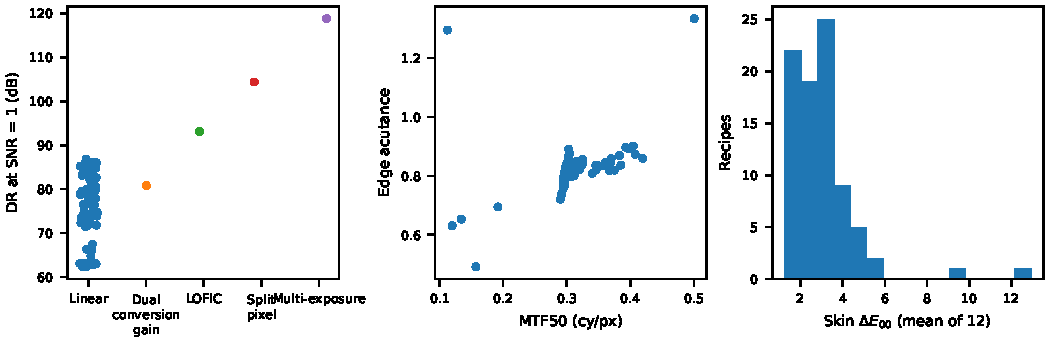
\includegraphics[width=0.9\textwidth]{figures/fig_scorecard.pdf}
\caption{Scorecard overview. Left: DR at SNR\,=\,1 by HDR architecture. Centre: MTF50 against edge acutance. Right: distribution of mean skin $\Delta E_{00}$ over recipes.}
\label{fig:sc}
\end{figure*}

\section{Discussion and limitations}
Three lessons from building the scorecard generalise to any simulated IQ comparison. First, a metric that is unbiased on laboratory captures is not automatically unbiased on simulation: noise-free inputs exposed the 4$\times$ binning bias in MTF50 that real noise would hide. Second, render noise must be kept apart from sensor noise: two captures with different sensor seeds separate them for SNR and DR, and texture metrics also need two independently seeded renders. Third, exposure and chart lighting are part of the measurement. A first full sweep metered only on the ColorChecker white, and it clipped the unevenly lit edge card on every linear recipe. That made the clipped linear sensors look sharper than the HDR pixels, which did not clip. Removing the clipping exposed the uneven lighting, which made MTF50 noise-driven. It also clipped the W channel of RGBW and the ADC of the binned quad-Bayer readout. None of these errors made a run fail, and the metric code was unbiased; only the implausible numbers exposed them. Fourth, ROIs must be found where the lens actually places the target, not where a pinhole would.

The limitations are explicit. P2020 and CPIQ implementations are uncertified. The synthetic skin tones are not measured population data. Colour correction uses each recipe's spectral ColorChecker matrix, so the skin result measures the sensor and its matrix, not a tuned ISP. pbrt's realistic camera traces no inter-reflections, so the veiling glare reported here excludes ghosts and coatings; open-cam models those separately~\cite{hullin2011flare} but the scorecard does not yet include them. The HDR chart excludes optics. The noise-free least-squares ColorChecker CCM of the RGBW recipe has a W coefficient of about 14, because $R+G+B\approx W$ makes the fit ill-conditioned. Its output edge and texture results therefore measure the unregularised matrix rather than the CFA itself; the sensor-domain sharpness isolates the CFA, and a regularised CCM or a separate luminance path is future work. At \scRes{} the slanted-edge ROI through the realistic lenses is only about 44\,px square, and its MTF ripples by about $\pm0.1$ between 0.2 and 0.4\,cy/px; where the curve hovers near 0.5, MTF50 can jump between neighbouring crossings (0.30 vs 0.40\,cy/px for two recipes behind the same lens), so edge acutance, which integrates the curve, is the more robust sharpness ranking. The two green sites of the Bayer recipes differ by about 7\,\% on the white patch. Many recipes carry EMVA parameters inferred from public tables rather than measured reports, so the scorecard ranks the recipes as modelled, not the cameras they are named after.

\section{Conclusion}
The open-cam IQ lab gives a reproducible path from spectral scenes to standard-style IQ numbers for any camera recipe, with every metric validated against closed-form ground truth before it is applied to renders. The scorecard, the validation suite and a lecture-oriented GUI share one code path, and all scripts behind this paper are at \url{https://github.com/briandeegan82/open-cam}.

\small
\bibliographystyle{ieeetr}
\bibliography{references}

\begin{biography}
Brian Deegan is with the University of Galway, Ireland. His research focuses on camera image quality, sensor and optics modelling, and simulation for automotive imaging.
\end{biography}

\end{document}
